\documentclass[12pt]{article}
\usepackage[margin=1in]{geometry}
\usepackage{amsfonts, amsmath, amssymb, amsthm, graphicx, booktabs}
\usepackage[none]{hyphenat}
\usepackage{fancyhdr}

\pagestyle{fancy}
\fancyhf{}
\fancyfoot[C]{\thepage}
% Uncomment the following if needed:
% \renewcommand{\headrulewidth}{0pt}
% \renewcommand{\footrulewidth}{0pt}

\begin{document}

\begin{titlepage}
\begin{center}
\vspace*{1cm}
\vfill
\line(1,0){400}\\[1mm]
\huge{\textbf{The Paradox of $\pi$}}\\[3mm]
\Large{\textbf{- The Finite and the Infinite -}}\\[1mm]
\line(1,0){400}
\vfill
By Takaya Ueno
\end{center}
\end{titlepage}

\section{Introduction}

\subsection{The History and Definition of $\pi$}
Abstractness is not a new concept at all in the field of mathematics. It is relatively straightforward to understand that mathematicians, especially those in the field of pure mathematics would attempt to push the boundaries that may seem alien to the real world. However, one number has always fascinated me \textendash not because of its existence, but because of how often it appears in real-world applications across many fields despite its seemingly "unrealistic" nature. I am talking about the famous $\pi$.\\

\noindent Let's consider a popular challenge involving $\pi$: how many digits of $\pi$ can you recite? Is it 10 digits? 100 digits? maybe even 1000? According to the Guinness World Records, \textbf{Rajveer Meena} holds the record for memorizing an astonishing \textbf{70,000 digits of $\pi$} \cite{guinness2017}. While this feat is nothing short of extraordinary, it barely scratches the surface, as $\pi$ continues infinitely.\\

\noindent This raises an important question: how can a value that never ends be used in real life? And who discovered $\pi$ in the first place? Let's take a brief journey through the history of $\pi$. \\

\noindent The earliest known approximations of $\pi$ come from the \textbf{Babylonians} (c. 1900-1600 BCE) where they calculated the area of a circle by taking three times the square of its radius, giving $\pi \approx 3$. They were also able to improve this approximation to $\frac{25}{8} = $ 3.125 \cite{exploratorium_pi}. Around the same time period, the \textbf{Ancient Egyptians} (c. 1650 BCE) , as recorded in the \textbf{Rhind Mathematical Papyrus} (written by the scribe \textbf{Ahmes}) approximated $\pi$ as $(\frac{16}{9})^2 \approx 3.16$ \cite{exploratorium_pi}. Nonetheless, the first to rigorously calculate the bounds of $\pi$ was done by one of the most famous mathematicians in history, \textbf{Archimedes of Syracuse} (c. 287 - 212 BCE). He achieved this by inscribing and circumscribing polygons around a circle. By increasing the number of sides of these polygons, Archimedes was able to narrow down the value of $\pi$ \cite{b2020archimedesshowedpiapproximately} (see Appendix A.1).\\

\noindent He established the following bounds for $\pi$:
\begin{center}
    $3\frac{10}{17} < \pi < 3\frac{1}{7}$
\end{center}
The following image illustrates this method by showing a circle with inscribed polygons of increasing sides, demonstrating how the polygons approach the shape of the circle more closely:
\begin{center}
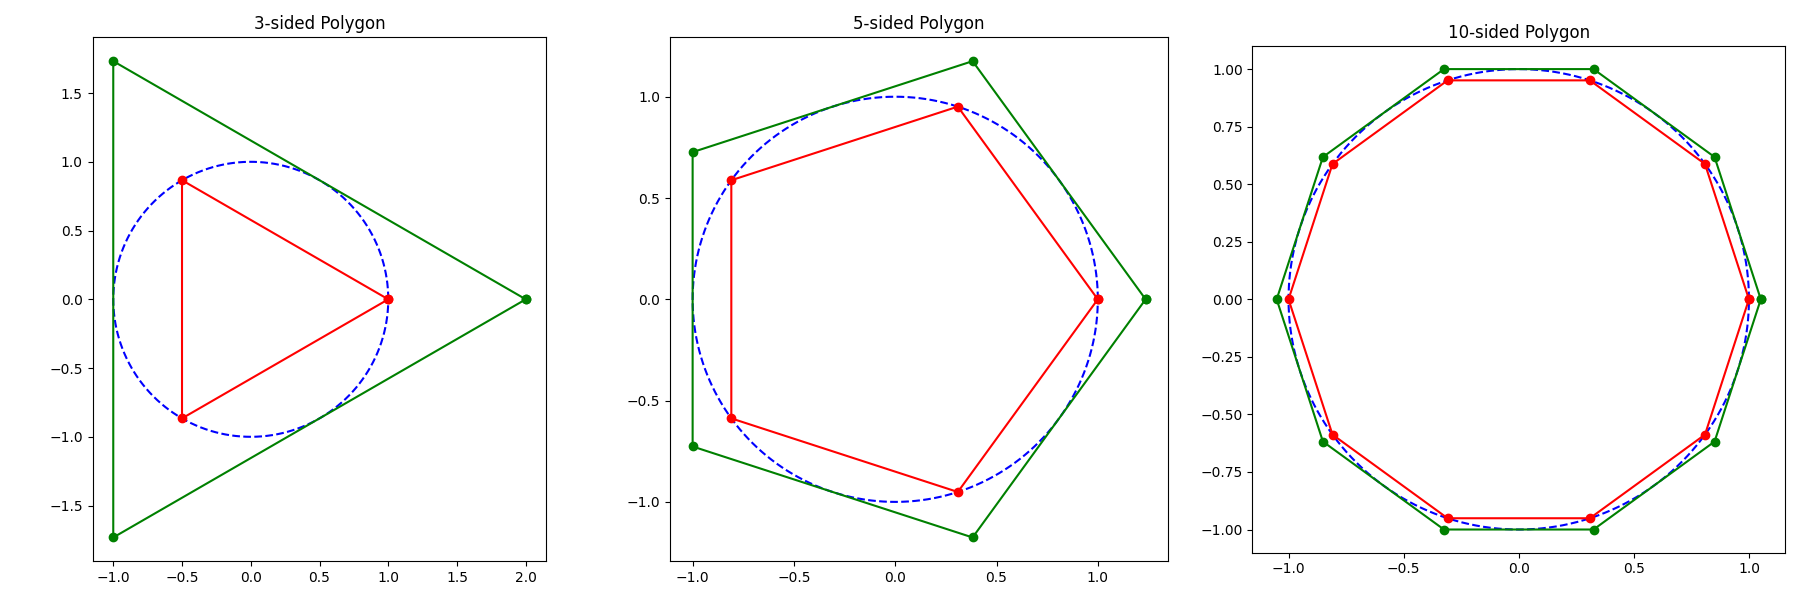
\includegraphics[width=1\textwidth]{images/Figure_1.png}
\end{center}

\noindent As the number of sides increases (e.g., triangles, pentagons, decagons), the polygons approximate the circumference of the circle more precisely. This technique laid the foundation for future numeral methods to approximate $\pi$. \\

\noindent Further down the line, we get closer to what we might all be familiar in the modern-day representation of $\pi$. In \textbf{Ancient China}, two figures made significant discoveries regarding $\pi$. Chinese mathematician \textbf{Liu Hui} (c. 3rd Century CE) used a 96-sided polygon and calculated $\pi$ to be approximately $3.14159$. Additionally, another mathematician, \textbf{Zu Chongzhi} (c. 5th Century CE) calculated $\pi$ to seven decimal places ($3.1415926$) and further gave a fractional approximation $\frac{355}{113}$, which remained highly accurate for around 1000 years after its discovery \cite{straffin1998}.  \\

\noindent Of course there is much more to the history of
$\pi$, but brief overview shows how the value of $\pi$ has evolved over time. Now, let's delve into the fascinating irrationality of $\pi$

\subsection{The Irrationality of $\pi$: Why Saying $\pi$ is Infinite Isn't Entirely Accurate}

\noindent Let's discuss what it means for a value to be \textbf{irrational}. An irrational number is simply a number that is \textbf{not rational}. In other words, it cannot be expressed as a ratio of two numbers (like $\frac{a}{b}$ where $a,b \in \mathbb{Z}$ and $b \neq 0$).\\

\noindent For example, consider the number $\sqrt{2}$. No matter how hard one tries, it is impossible to express $\sqrt{2}$ as a simple fraction like $\frac{p}{q}$. The decimal expansion of this value goes on forever without repeating (see Appendix A.2):
\begin{center}
    $1.41421356\ldots$
\end{center}
This \textbf{non-repeating, non-terminating} nature is the defining feature of irrational numbers.\\

\noindent The number $\pi$ also shares this property. In \textbf{1768}, \textbf{Johann Lambert} proved that $\pi$ is irrational \cite{Denis}, to which \textbf{Miklós Laczkovich} gave a more modern and accessible proof in $1997$ (see Appendix A.3). This means that there is no fraction $\frac{a}{b}$ that equals $\pi$ exactly. Its decimal expansion goes on forever without ever settling into a repeating pattern:
\begin{center}
    $\pi = 3.14159265358979\ldots$
\end{center}

\noindent However, it is very important to clarify what we mean when we say that $\pi$ is infinite. This itself is in fact \textbf{flawed} since the number $\pi$ is \textbf{finite}\textendash it has a definite value. What is \textbf{infinite} is its \textbf{decimal representation}. The distinction between the two is crucial.

\subsection{Finite Value vs. Infinite Representation}

\noindent When dealing with numbers like $\pi$ or $\sqrt{2}$, it is essential to understand the distinction between their \textbf{finite values} and their \textbf{infinite decimal representations}. At first glance, this may seem contradictory, but the distinction is fundamental to understanding irrational numbers.\\

\noindent A \textbf{finite value} refers to a specific, well-defined quantity. This does not necessarily mean it can be expressed fully in decimal form, but rather, the number represents a unique point on the number line. For example:
\begin{itemize}
    \item The number $\pi$ is the exact ratio of the circumference of a circle to its diameter.
    \item The number $\sqrt{2}$ is the exact length of the diagonal of a square with the sides having a length of 1.
\end{itemize}

\noindent On the other hand, an \textbf{infinite decimal representation} is a way of expressing a number in the decimal system where the digits go on forever without terminating. This occurs frequently with irrational numbers, which cannot be written as a fraction of two integers. Examples include:

\begin{enumerate}
    \item $\pi = 3.141592653589793\ldots$ (non-repeating)
    \item $\sqrt{2} = 1.41421356237\ldots$ (non-repeating)
    \item Even rational numbers like $\frac{1}{3} = 0.3333\ldots$ have infinite, repeating decimals
\end{enumerate}

\noindent Despite their infinite decimal expansions, numbers like $\pi$ or $\sqrt{2}$ represents a definite, finite quantity. For instance, the circumference of a circle with a diameter of 1 unit is exactly $\pi$ units. This value is finite, fixed and does not change.\\

\noindent It is remarkable how finite values (even certain rational numbers) can have infinite decimal expressions. But why does this happen? The answer lies in the limitations of the \textbf{base-10 decimal system} we use. \\

\noindent In a \textbf{base-10} system, we represent numbers using powers of 10. When converting a number into a decimal format, we express it as a sum of these powers. For example, the decimal $2.136$ means:
\begin{center}
    $2 \times 10^0 + 1 \times 10^{-1} + 3 \times 10^{-2} + 6 \times 10^{-3}$
\end{center}
However, not all numbers can be perfectly expressed as finite sums of these powers of 10. This is a limitation of the \textbf{decimal system}, not of the numbers themselves.\\

\noindent Interestingly, there are other \textbf{number bases} where a value can be represented finitely, even if it cannot be done in base-10. For example, in base-10:
\begin{center}
    $\frac{1}{3} = 0.3333333 \ldots$
\end{center}

\noindent However, in \textbf{base-3} (also called ternary), this same fraction has a finite representation:
\begin{center}
    $\frac{1}{3} = 0.1_3$
\end{center}

\noindent This works because 3 divides evenly into powers of 3, making the division exact and finite in base-3. Conversely, the values that have finite representations in base-10 may have infinite representations in other bases.\\

\noindent Now that we have established the distinction between finite values and infinite decimal representations, consider the following analogy to better understand this concept.\\

\noindent \textbf{Analogy: Measuring a Rope}\\

\noindent Suppose you have a rope that is exactly $\pi$ meters long. The rope itself has a definite, finite length. It does not stretch into infinity\textendash it is precisely $\pi$ meters long. However, if you try to measure it using increasingly precise units (e.g., meters, centimeters, millimeters, micrometers), you can keep expressing the length with more decimal places:
\begin{center}
    $3.1$m, \ $3.14$m, \ $3.141$m, \ $3.1415$m $\ldots$
\end{center}
You can never write down the \textit{exact} length in decimal form since the digits go on forever. However, this does not mean that the rope itself is becoming increasingly longer as you add more decimal places. 

\section{Applications}

\subsection{Ratio of a Circle's Circumference}
There have already been previous mentions of $\pi$ as the ratio of a circle's circumference. Here, I will go a little more in depth and explain how this relationship is applicable in the real world.\\

\noindent $\pi$ is fundamentally defined as the ratio of a circle's circumference $C$ to its diameter $d$:
\begin{center}
    $\pi = \frac{C}{d}$
\end{center}

\noindent Thus, the circumference of a circle can be expressed as:
\begin{center}
    $C = \pi d = 2\pi r$
\end{center}
where \(r\) is the radius of a circle.\\

\noindent The relationship between $\pi$ and a circle is fundamental to the fields of \textbf{geometry} and \textbf{trigonometry}. This relationship is used in various applications such as calculating the length of circular objects (e.g., wheels, pipes) and designing structures with circular features (e.g., domes, arenas). Despite $\pi$'s infinite decimal expansion, we can use approximations like $3.14$ or $22/7$ to achieve precise enough measurements for real-world applications.\\

#### \textbf{Examples of Real-World Applications}
\begin{enumerate}
    \item \textbf{Engineering and Architecture}:
    Calculating the circumference or perimeter of circular structures such as tunnels or bridges. For example, if an architect designs a circular section of a park with a diameter of 10 meters, the circumference is
    \begin{center}
        $C = \pi \times 10 \approx 31.42$ meters
    \end{center}
    \item \textbf{Manufacturing}:
    Producing gears and wheels where precise measurements of circular dimensions are important. A bicycle wheel with a radius of $0.35$ meters has a circumference of:
    \begin{center}
        $C = 2\pi \times 0.35 \approx 2.2$ meters.
    \end{center}
    \item \textbf{Astronomy}:
    Determining planetary orbits and calculating the circumferences of celestial bodies. For instance, the Earth's equatorial diameter is about $12,742$km, making its circumference approximately:
    \begin{center}
        $C = \pi \times 12,742 \approx 40,030$km
    \end{center}
\end{enumerate}
% Waves and Oscillations %
\subsection{Waves and Oscillations}

$\pi$ also appears naturally in the study of \textbf{waves} and \textbf{oscillations} due to their periodic nature. Functions like sine and cosine describe wave behaviors and are intimately connected with $\pi$,
\begin{center}
    $y = \sin\theta, \ y = \cos\theta$
\end{center}
where $\theta$ is the angle measured in \textbf{radians}, and one full cycle corresponds to $2\pi$ radians (equivalent to $360^\circ$)\\

#### \textbf{Wave Properties Involving $\pi$}

\begin{enumerate}
    \item \textbf{Period of a Wave}: The \textbf{period} $T$ is the time it takes for a wave to complete one cycle. For a sine wave, the period is typically related to $2\pi$. The general equation for a wave can be expressed as:
    \begin{center}
    $y(t) = A\sin\left(\frac{2\pi}{T}t\right)$
    \end{center}
    where $A$ is the amplitude and $t$ is time.
    \item \textbf{Angular Frequency}:
    The \textbf{frequency} $f$ is the number of cycles per second. The \textbf{angular frequency} $\omega$ of a wave is given by:
    \begin{center}
    $\omega = 2\pi f$
    \end{center}
    where $f$ is the number of oscillations per second.  
\end{enumerate}
#### \textbf{Examples of Real-World Applications}:
\begin{enumerate}
    \item \textbf{Musical Notes}: Musical notes are produced by vibrating strings (such as on a violin or guitar) or air columns (as in brass instruments). The pitch of a note depends on the frequency of the wave, which involves $\pi$. For example, a tuning fork vibrating at $440$Hz, which is the note A, can be described by the function:
    \begin{center}
        $y(t) = A\sin(2\pi \times 440\times t)$.
    \end{center}
    \item \textbf{Electromagnetic Waves}:
    Light, radio waves and microwaves oscillate at very high frequencies. These waves are described using sine and cosine functions involving $\pi$. For a plane electromagnetic wave traveling in the $x$-direction, the electric field $E$ and magnetic field $B$ can be expressed as:
    \begin{center}
        $E(x,t) = E_0\sin(kx - wt)\hat{j}$ \\ \vspace{3mm}
        $B(x,t) = B_0 \sin(kx - wt)\hat{k}$
    \end{center}
    Where:
    \begin{itemize}
        \item $E_0$ is the amplitude of the electric field.
        \item $B_0$ is the amplitude of the magnetic field.
        \item $k = \frac{2\pi}{\lambda}$ is the wave number such that $\lambda$ is the wave length.
        \item $\omega = 2\pi f$ is the angular frequency, where $f$ is the frequency (as shown previously).
        \item $x$ is the position in space.
        \item $t$ is time and $\hat{j}, \ \hat{k}$ are unit vectors indicating the directions of the fields.
    \end{itemize}
    \begin{center}
        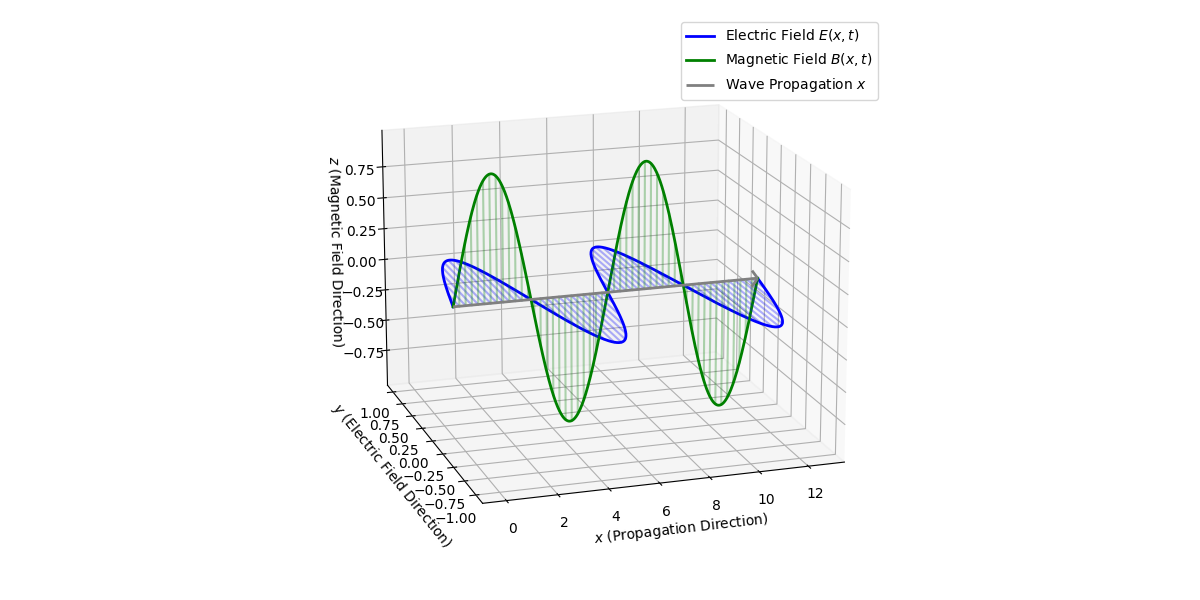
\includegraphics[width=1\textwidth]{images/Figure_2.png}
    \end{center}
    \noindent In summary, the electric field $E(x,t)$ oscillates in the $y$-direction $(\hat{j})$, the magnetic field $B(x,t)$ oscillates in the $z$-direction $(\hat{k})$ and the wave propagates in the $x$-direction.
\end{enumerate}

\section{The Finite and the Infinite}

\subsection{$\pi$ as a Bridge Between the Finite and Infinite}

\noindent The number $\pi$ uniquely illustrates how mathematics connects the \textbf{finite world} we experience to the \textbf{infinite complexities} underlying it. Though $\pi$ has an \textbf{infinite decimal expansion}, it represents something very \textbf{concrete and finite}. \\

\noindent An interesting geometric paradox arises from a \textbf{perfect circle}. Its boundary is smooth, finite and easy for anyone to visualize. Yet, the number needed to describe its exact circumference is \textbf{infinitely complex}. This paradox beautifully demonstrates how simple, finite shapes can hide \textbf{infinite mathematical depth}. \\

\noindent I have yet to discuss, due to its complex nature, but the infinite nature of $\pi$ becomes even more evident in its representation through what is known as an infinite series, which is a sum of values that never ends:
\begin{center}
    $\pi = 4 \sum\limits_{n=0}^\infty \frac{(-1)^n}{2n + 1} = 4\left(1 - \frac{1}{3} + \frac{1}{5} - \frac{1}{7} + \ldots\right)$ \quad [7]
\end{center}
The above is the \textbf{Leibniz series}, which shows that calculating the exact value of $\pi$ requires the summation of an infinite number of terms. It highlights how the \textbf{finite value} of $\pi$ is intrinsically tied to a \textbf{never-ending process}.

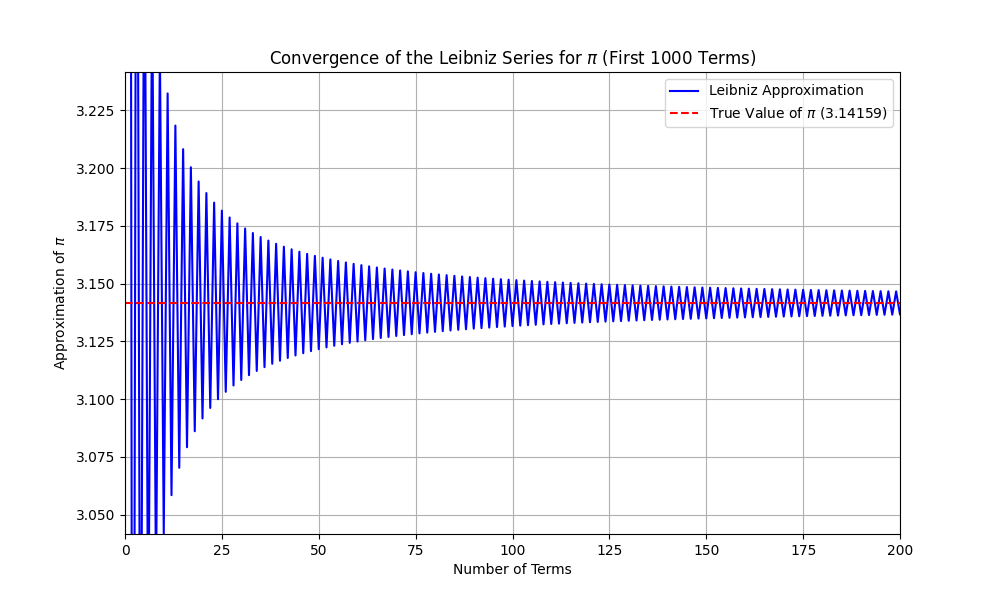
\includegraphics[width=1\textwidth]{images/Figure_3.png}

\noindent The above figure shows that the more terms you add to the Leibniz series, the closer and closer you get to the true value of $\pi$.

\subsection{Practicality vs Precision}
While $\pi$ has an infinite decimal expansion, in practice, we rarely need its full precision as shown in some of the real-world examples. This balance between \textbf{practicality} and \textbf{precision} shows how we harness the infinite nature of $\pi$ for the use of finite, real-world purposes.\\

\noindent The level of precision required depends on the application:

\begin{itemize}
    \item \textbf{Space Exploration}: NASA typically uses $\pi$ to about \textbf{$15$ decimal places} for spacecraft navigation. This precision is necessary for calculating the trajectory of spacecraft traveling millions of kilometers in space \cite{nasa_pi}.
    \item \textbf{Everyday Applications}: For most day-to-day calculations, \textbf{two decimal places} ($\pi \approx 3.14)$ are sufficient. For example, calculating the circumference of a dinner plate or a roundabout does not require extreme precision required for space exploration.
    \item \textbf{Engineering}: In fields like civil and mechanical engineering, $\pi$ is often used to \textbf{four to five decimal places} when constructing large circular structures. This level of accuracy ensures that calculations are precise enough for practical use.
\end{itemize}

\noindent In \textbf{pure mathematics} and research, computing $\pi$ to \textbf{trillions of digits} serves to test the limits of computational power and explore mathematical theory rather than to solve practical problems.\\

\noindent Despite the infinite complexities of $\pi$, it can still be approximated with remarkable accuracy. In fact, in many real-world situations, using too many decimal places for $\pi$ often results in diminishing returns. The additional precision becomes effectively meaningless compared to other more prominent factors such as \textbf{material imperfections} or \textbf{measurement errors}. This balance between practicality and precision truly highlights how mathematics, while abstract, can be applied effectively to solve concrete, finite problems. 

\newpage

\appendix

\section{Idea Behind the Proofs}

\subsection{Archimedes' Method for Approximating $\pi$}

\noindent Let $C$ be the circumference of a circle with radius $r$. The circumference is related to $\pi$ by $C = 2\pi r$.\\

\noindent Archimedes used regular polygons with $n$ sides inscribed inside and circumscribed outside the circle. Let $C_n$ be the circumscribed polygon and $c_n$ be the inscribed polygon such that:
\begin{center}
    $c_n < C < C_n$
\end{center}
\begin{center}
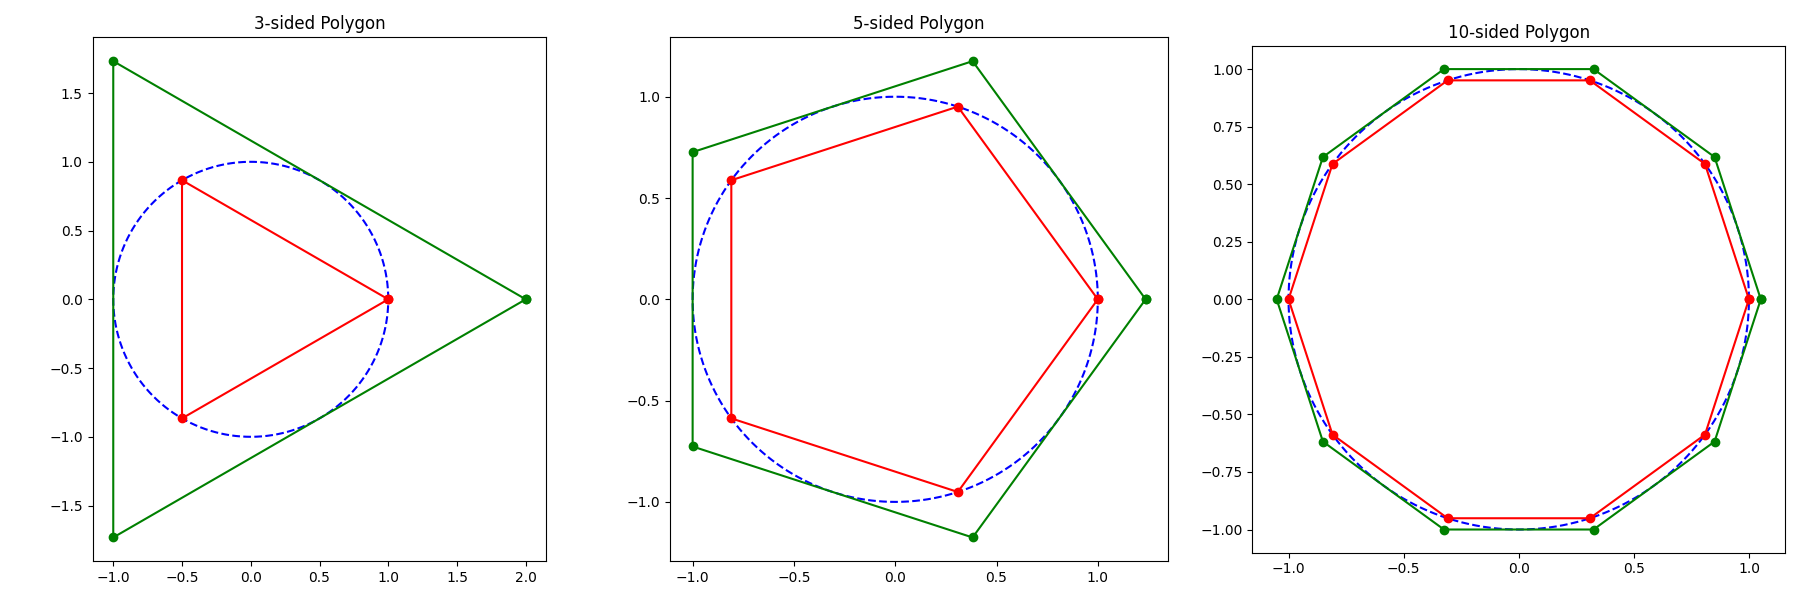
\includegraphics[width=1\textwidth]{images/Figure_1.png}
\end{center}
It is clear from the figure above that the decagon (or $10-$gon) has a circumference that is closest to the circle.\\

\noindent Thus, we can find an accurate value of $\pi$ by taking some large $n$, but rather than brute forcing through every possible value of $n$, Archimedes doubled the number of sides. \\

\noindent To calculate the side length of new polygon when doubling the sides, Archimedes used the \textbf{Pythagorean theorem}. Let $s_n$ be the side length of a polygon with $n$ sides, then the side length $s_{2n}$ of a polygon with $2n$ sides can be determined using the formula:
\begin{equation}
    s_{2n} = \sqrt{2-\sqrt{4-s^2_n}}
    \label{eq:doubling_formula}
\end{equation}
This formula comes from the geometry of the circle and the triangles formed within the inscribed polygon.\\

\noindent Start with a hexagon where $n = 6$. For a circle of radius $r = 1$, the side length $s_6$ of the inscribed hexagon is:
\begin{center}
    $s_6 = 2\sin(\frac{\pi}{6}) = 1$
\end{center}
The use of $\sin(\frac{\pi}{6})$ might seem counterintuitive since it seems that we are approximating $\pi$ by using $\pi$, but this value comes from the known geometric property of a hexagon inscribed in a unit circle.\\

\noindent We can then double this by using equation \ref{eq:doubling_formula}:
\begin{equation}
    s_{12} = \sqrt{2 - \sqrt{4 - s_6^2}} = \sqrt{2 - \sqrt{4 - 1^2}} = \sqrt{2 - \sqrt{3}}
\end{equation}
By continuing this process, we get:
\begin{equation}
    s_{96} = \sqrt{2 - \sqrt{4 - s_{48}^2}}
\end{equation}
After calculating the perimeters of the inscribed and circumscribed polygons for a $96$-sided polygon, Archimedes found the following bounds for $\pi$:
\begin{center}
    $3 \frac{10}{71} < \pi < 3\frac{1}{7}$
\end{center}
or in decimal form:
\begin{center}
    $3.1408 < \pi < 3.1429$
\end{center}
We can also take a look at the following table of approximations to see that the approximation error gets increasingly smaller:
\subsection*{Table of Approximations}

\begin{center}
    \begin{tabular}{cccc}
        \toprule
        \textbf{Iterations} & \textbf{Sides} & \textbf{Result} & \textbf{Error} \\
        \midrule
        0  & 4     & 2.8284271247 & -0.3131655288 \\
        1  & 8     & 3.0614674589 & -0.0801251947 \\
        2  & 16    & 3.1214451523 & -0.0201475013 \\
        3  & 32    & 3.1365484905 & -0.0050441630 \\
        4  & 64    & 3.1403311570 & -0.0012614966 \\
        5  & 128   & 3.1412772509 & -0.0003154027 \\
        6  & 256   & 3.1415138011 & -0.0000788524 \\
        7  & 512   & 3.1415729404 & -0.0000197132 \\
        8  & 1024  & 3.1415877253 & -0.0000049283 \\
        9  & 2048  & 3.1415914215 & -0.0000012321 \\
        10 & 4096  & 3.1415923456 & -0.0000003080 \\
        \bottomrule
    \end{tabular}
\end{center}

\noindent For a more detailed explanation, see: \textbf{Damini D.B and Abhishek Dhar}. \textit{How Archimedes show that $\pi$ is approximately equal to $\frac{22}{7}$} \cite{b2020archimedesshowedpiapproximately}. 


\subsection{Euclid's Proof of the Irrationality of $\sqrt{2}$}

\noindent \textbf{Statement:} The square root of $2$ is irrational.\\

\noindent Properties of Fractions and Even Numbers:
\begin{enumerate}
    \item If you take any number and multiply it by $2$, the result must be even.
    \item If the square of a number is even, the number itself must be even.
    \item Fractions can be simplified (e.g., $\frac{12}{8} = \frac{3}{2}$). However, it is impossible to simplify a fraction forever.
\end{enumerate}

\begin{proof}
\noindent Assume that $\sqrt{2}$ is a rational number. That is, it can be written in the form:
\begin{center}
    $\sqrt{2} = \frac{p}{q}$ where $p, q \in \mathbb{Z}$
\end{center}
By squaring both sides, we get:
\begin{center}
    $2 = \frac{p^2}{q^2}$
\end{center}
Rearranging the terms gives:
\begin{center}
    $2q^2 = p^2$
\end{center}
By property \textbf{1}, we know that $p^2$ must be even. Moreover, from property \textbf{2}, $p$ must also be even. We can then write it as $2m$, where $m$ is some whole number. Thus we get the following:
\begin{center}
    $2q^2 = (2m)^2 = 4m^2$
\end{center}
Divide both sides by $2$:
\begin{center}
    $q^2 = 2m^2$
\end{center}
Again, by the same arguments used before, $q^2$ and $q$ must also be even. We can write $q$ as $2n$ for some whole number $n$.
\begin{center}
    $\sqrt{2} = \frac{p}{q} = \frac{2m}{2n}$
\end{center}
This can then be simplified by dividing both the numerator and denominator by 2.
\begin{center}
    $\sqrt{2} = \frac{m}{n}$
\end{center}
The above equation is now in a simpler form than the initial $\frac{p}{q}$. However, we can repeat this exact same process on $\frac{m}{n}$, thus generating an even simpler fraction, to which we can also repeat the same process over and over again.\\

\noindent This implies that there is an infinite number of simplifications, which by property \textbf{3}, is impossible. There must always be a simplest fraction.\\

\noindent Hence, $\sqrt{2}$ is irrational by contradiction \cite{singh1997fermat}.

\end{proof}


\subsection{Laczkovich's Proof of the Irrationality of $\pi$}
\begin{proof}
Suppose, for contradiction, that $\pi$ is rational. That is $\pi = \frac{p}{q}$, where $p, q \in \mathbb{Z}$.\\

\noindent Consider the Taylor series for $\sin(x)$. The sine function has the following Taylor series expansion around $x = 0$:
\begin{equation}
    \sin(x) = x - \frac{x^3}{3!} + \frac{x^5}{5!} - \frac{x^7}{7!} + \ldots = \sum_{n=0}^\infty (-1)^n \frac{x^{2n+1}}{(2n+1)!}
\end{equation}
Plugging $\pi = \frac{p}{q}$ into the Taylor series gives:
\begin{equation}
    \sin\left(\frac{p}{q}\right) = \frac{p}{q} - \frac{\left(\frac{p}{q}\right)^3}{3!} + \frac{\left(\frac{p}{q}\right)^5}{5!} - \ldots
\end{equation}
We know that $\sin(\pi) = 0$. Hence, the infinite sum must equal zero:
\begin{equation}
    0 = \frac{p}{q} - \frac{\left(\frac{p}{q}\right)^3}{3!} + \frac{\left(\frac{p}{q}\right)^5}{5!} - \ldots
\end{equation}
We can then rewrite the equation by multiplying both sides by $q^{2n+1}$ to clear the denominators of $\frac{p}{q}$:
\begin{equation}
    0 = pq^{2n} - \frac{p^3q^{2n-2}}{3!} + \frac{p^5q^{2n-4}}{5!} - \ldots
\end{equation}
Observe that the right-hand side is an infinite sum of terms involving integers, alternating in sign. However, also notice that this sum cannot equal zero unless $p = 0$, which contradicts the initial assumption that $\pi = \frac{p}{q}$ is a non-zero value.\\

\noindent Hence, $\pi$ is not rational and must be irrational.

\end{proof}

\noindent For a more detail explanation, see: 
\textbf{Laczkovich, M. (1997)}. \textit{On Lambert's proof the irrationality of $\pi$}. \textbf{American Mathematical Monthly, 104(5), 439-443} \cite{Laczkovich1997}.

\subsection{Leibniz's Series for $\pi$}

The Leibniz series for $\pi$ is given by:
\begin{center}
    $\pi = 4 \left(1 - \frac{1}{3} + \frac{1}{5} - \frac{1}{7} + \frac{1}{9} - \ldots\right) = 4
    \sum\limits_{n=0}^\infty \frac{(-1)^n}{2n + 1}$
\end{center}
This series expresses $\pi$ as an alternating sum of fractions involving odd values.\\

\noindent The above series can be derived from the Taylor series expansion of the arctangent function $\arctan(x)$:

\begin{equation}
    \arctan(x) = \sum_{n=0}^\infty (-1)^n\frac{x^{2n+1}}{2n+1}, \text{ for } |x| \leq 1
\end{equation}

\noindent In the special case $\arctan(1)$, we know that:
\begin{center}
    $\arctan(1) = \frac{\pi}{4}$
\end{center}
Substitute $x = 1$ into the Taylor series for $\arctan(x)$ gives:
\begin{center}
    $\frac{\pi}{4} = \sum\limits_{n=0}^\infty (-1)^n \frac{1}{2n+1}$
\end{center}
Multiply both sides by 4, we get the Leibniz series:
\begin{center}
    $\pi = 4\sum\limits_{n=0}^\infty \frac{(-1)^n}{2n+1}$
\end{center}

\noindent The alternating nature of the series ensures that the partial sums get closer and closer to $\pi$ as more terms are added.\\

\noindent Although the Leibniz series works, it converges very slowly. This slow implies that a large number of terms are required to get an accurate approximation of $\pi$.\\

\noindent Observe the following and how the increasing number of terms improves the approximation:
\begin{center}
    $\pi \approx 4(1) = 4.0000$ (Error: $0.8584$)\\
    \vspace{3mm}
    $\pi \approx  4\left(1 - \frac{1}{3} + \frac{1}{5}\right) = 3.4667$ (Error: 0.3251)\\
    \vspace{3mm}
    $\pi \approx 4\left(1 - \frac{1}{3} + \frac{1}{5} - \frac{1}{7} + \frac{1}{9} - \frac{1}{11} + \frac{1}{13}\right) = 3.2840$ (Error: 0.1424)\\
    \vspace{3mm}
    $\pi \approx 4\left(1 - \frac{1}{3} + \frac{1}{5} - \frac{1}{7} + \frac{1}{9} - \frac{1}{11} + \frac{1}{13} - \frac{1}{15} + \frac{1}{17} - \frac{1}{19}\right) = 3.0416$ (Error: $-0.1000$)
\end{center}
The slow convergence occurs due to the terms $\frac{1}{2n+1}$ decreases very gradually. In other words, each additional term only makes a small adjustments to the overall sum. The Leibniz series is often used to introduce concepts of infinite series and alternating series in calculus and real analysis courses. \\

\noindent For a more detailed explanation, see: \textbf{Wikipedia contributors}. \textit{Leibniz formula for $\pi$}. \textbf{Wikipedia, The Free Encyclopedia} \cite{wikipedia_leibniz}. 

\newpage

\bibliographystyle{plain}
\bibliography{references}

\end{document}
